\documentclass[10pt,a4paper]{article}
\usepackage[utf8]{inputenc}
\usepackage[T1]{fontenc}
\usepackage{lmodern}
\usepackage[margin=1.7cm]{geometry}
\usepackage{titlesec}
\titlespacing*{\section}{0pt}{0.9em}{0.4em}
\usepackage{booktabs}
\usepackage{tabularx}
\usepackage{xcolor}
\usepackage{tikz}
\usetikzlibrary{positioning,arrows.meta,fit,backgrounds,calc}
\usepackage[hidelinks]{hyperref}
\usepackage{enumitem}
\setlist{nosep,leftmargin=1.2em}
\setlength{\parskip}{0.35em}
\setlength{\parindent}{0pt}

\definecolor{llm}{HTML}{E0B37B}
\definecolor{llmline}{HTML}{8A6A3F}
\definecolor{code}{HTML}{D3EDF5}
\definecolor{codeline}{HTML}{285971}
\definecolor{data}{HTML}{0B3F4D}

\title{\vspace{-1.6em}\textbf{RAGstofan}\\[0.2em]\large Asking Statistics Iceland in plain English or Icelandic}
\author{Gagnaþon 2026 \textperiodcentered{} Track 2: an agentic AI over Statistics Iceland's PX-API}
\date{\vspace{-1.2em}}

\begin{document}
\maketitle
\vspace{-0.8em}

\section*{What we set out to do}

Statistics Iceland (Hagstofa Íslands) publishes 1,857 tables through its PX-API. The numbers are there, but finding
them means knowing which table holds them, which of its dimensions and categories to choose, and often doing a
calculation on top. RAGstofan lets anyone ask in plain English or Icelandic (``\emph{Hve mörgum fleiri karlar en
konur búa á Íslandi?}'') and get back the official figure, its unit, the table it came from with a link, a chart,
and every step that produced it.

Our goals were:
\begin{itemize}
  \item \textbf{The right number from the right official table}, for questions in either language.
  \item \textbf{Never an invented number.} The language model reads, plans and chooses; Python does every
        calculation, and every number in the written answer is checked against the data before it is shown.
  \item \textbf{Transparent answers}: the source table, the categories chosen, any calculation and each step's time
        are shown, so a user can check them.
  \item \textbf{Open models only}: any OpenAI-compatible endpoint. We ran Qwen models through Ollama on a GB10 GPU
        server (``the Spark''); the same code runs on a laptop.
\end{itemize}

\section*{How it works}

Figure~\ref{fig:arch} shows the path of a question. A language model is used only where judgement is needed (gold
boxes); everything that can be checked is done in code (blue).

\begin{enumerate}
  \item \textbf{Understand.} A follow-up (``and last year?'') is rewritten into a question that stands alone. A
        planner restates the question in English with search words and reads its facts: places, period and the
        breakdown wanted. Code drops any fact that is not in the user's own words.
  \item \textbf{Find the table, one table first.} The whole question is first treated as one part. Three methods each
        suggest a table, and the model confirms or rejects each with a yes or no: a hand-written \emph{keyword
        dictionary} of 212 subjects (\emph{verðbólga} $\rightarrow$ consumer price index $\rightarrow$ VIS01000);
        \emph{search} over all tables, with BM25 keyword search and multilingual e5 vectors run in parallel and fused
        by rank, after code rules drop variants nobody asked for; and \emph{every table}, where the model names its
        best three from a list of all tables sized to its context window. If no table is confirmed, the question is
        split into 2, 3 and then 4 parts; if a part still has none, the user picks from each method's top three.
  \item \textbf{Read the numbers.} The model chooses the categories (year, place, sex, \dots). Code checks every
        choice against the table, fills defaults (the total, the latest period) and applies the user's words (only
        the places named, quantity or value).
  \item \textbf{Calculate in code}: differences, percentage changes, shares, sums, rankings, highest and lowest, and
        figures per inhabitant across two tables.
  \item \textbf{Answer.} The chart type follows the shape of the data. The model writes one to three sentences; if
        any number in them is not in the data, a template written from the data replaces the answer. A last check
        reads the answer back against the question and says so up front when it is unsure.
\end{enumerate}

\textbf{Connection to Statistics Iceland.} A crawler walked the PX-API's table tree once and stored every table's
ID, titles in both languages, dimensions, periods and category labels (the catalogue that search runs over). For a
chosen table the app sends a \texttt{GET} for its metadata and a \texttt{POST} asking only for the categories needed,
in json-stat2 format, to \texttt{https://px.hagstofa.is/pxen/api/v1/en/<path>/<table>.px}. Calls are spaced at least
one second apart, retried on \texttt{429}, and cached. By default the same documents are read from the organisers'
snapshot of every table (18 October 2026), and the live API is asked only for tables or periods the snapshot lacks.

\textbf{Interfaces.} A website with charts and voice input, an HTTP API including the Track~2 endpoint
\texttt{/spyrja\_px\_api}, an iPhone and iPad app, and an MCP server so Claude, ChatGPT and other agents can call it.

\begin{figure}[t]
\centering
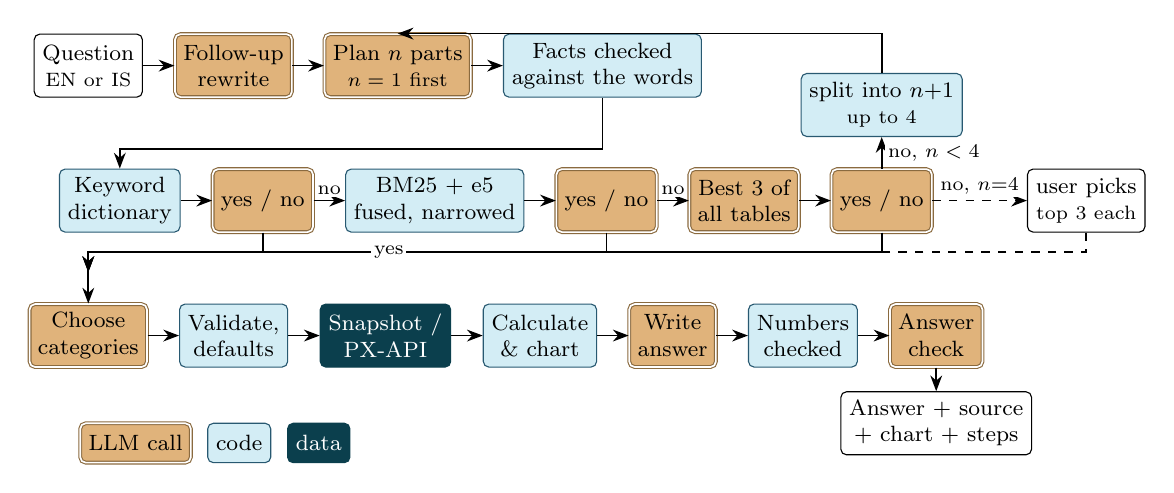
\begin{tikzpicture}[
  font=\footnotesize, node distance=3.5mm and 4mm,
  box/.style={draw, rounded corners=2pt, align=center, inner sep=3pt, minimum height=8mm},
  llm/.style={box, fill=llm, draw=llmline, double, double distance=0.6pt},
  code/.style={box, fill=code, draw=codeline},
  dat/.style={box, fill=data, text=white, draw=data},
  check/.style={code, diamond, aspect=2.2, inner sep=1pt},
  arr/.style={-{Stealth[length=2mm]}, semithick},
  lab/.style={font=\scriptsize, fill=white, inner sep=1pt}
]
% row 1: understand
\node[box, fill=white] (q) {Question\\\scriptsize EN or IS};
\node[llm, right=of q] (fu) {Follow-up\\rewrite};
\node[llm, right=of fu] (plan) {Plan $n$ parts\\\scriptsize $n=1$ first};
\node[code, right=of plan] (facts) {Facts checked\\against the words};
% row 2: find
\node[code, below=9mm of q, xshift=4mm] (dict) {Keyword\\dictionary};
\node[llm, right=of dict] (y1) {yes / no};
\node[code, right=of y1] (search) {BM25 + e5\\fused, narrowed};
\node[llm, right=of search] (y2) {yes / no};
\node[llm, right=of y2] (all) {Best 3 of\\all tables};
\node[llm, right=of all] (y3) {yes / no};
% row 3: read and answer
\node[llm, below=9mm of dict, xshift=-4mm] (cat) {Choose\\categories};
\node[code, right=of cat] (val) {Validate,\\defaults};
\node[dat, right=of val] (px) {Snapshot /\\PX-API};
\node[code, right=of px] (calc) {Calculate\\\& chart};
\node[llm, right=of calc] (write) {Write\\answer};
\node[code, right=of write] (num) {Numbers\\checked};
\node[llm, right=of num] (chk) {Answer\\check};
% side outcomes
\node[code, above=4mm of y3] (split) {split into $n{+}1$\\\scriptsize up to 4};
\node[box, fill=white, right=12mm of y3] (ask) {user picks\\\scriptsize top 3 each};
% arrows row 1
\draw[arr] (q) -- (fu); \draw[arr] (fu) -- (plan); \draw[arr] (plan) -- (facts);
\draw[arr] (facts.south) |- ($(dict.north)+(0,2.5mm)$) -- (dict.north);
% arrows row 2
\draw[arr] (dict) -- (y1);
\draw[arr] (y1) -- node[lab, above=1pt]{no} (search);
\draw[arr] (search) -- (y2);
\draw[arr] (y2) -- node[lab, above=1pt]{no} (all);
\draw[arr] (all) -- (y3);
\draw[arr] (y3.north) -- node[lab, right=1pt]{no, $n<4$} (split.south);
\draw[arr] (split.north) |- (plan.north);
\draw[arr, dashed] (y3) -- node[lab, above=1pt]{no, $n{=}4$} (ask);
% yes to categories
\coordinate (yes) at ($(cat.north)+(0,4mm)$);
\draw[arr] (y1.south) -- ++(0,-2.5mm) -| (yes) -- (cat.north);
\draw[arr] (y2.south) -- ++(0,-2.5mm) -| (yes);
\draw[arr] (y3.south) -- ++(0,-2.5mm) -| (yes);
\draw[arr, dashed] (ask.south) -- ++(0,-2.5mm) -| (yes);
\node[lab] at ($(y1.south)+(1.6,-0.25)$) {yes};
% arrows row 3
\draw[arr] (cat) -- (val); \draw[arr] (val) -- (px); \draw[arr] (px) -- (calc);
\draw[arr] (calc) -- (write); \draw[arr] (write) -- (num); \draw[arr] (num) -- (chk);
\node[box, fill=white, below=3mm of chk] (out) {Answer + source\\+ chart + steps};
\draw[arr] (chk) -- (out);
% legend
\node[llm, minimum height=5mm, below=7mm of cat, xshift=6mm] (kl) {LLM call};
\node[code, minimum height=5mm, right=2mm of kl] (kc) {code};
\node[dat, minimum height=5mm, right=2mm of kc] (kd) {data};
\end{tikzpicture}
\caption{RAGstofan's pipeline. Each part of a question goes through the table finder (middle row) in parallel; a
yes from any method, or the user's pick, leads to reading the numbers (bottom row). Python does all arithmetic.}
\label{fig:arch}
\end{figure}

\section*{Results}

\textbf{Benchmark.} We measured against the organisers' 60 questions over Statistics Iceland's data (release of
18 October 2026): 20 easy, 20 medium and 20 hard, each asked in English and Icelandic, with official answers. An
answer counts as right only if its number matches the official one; ``right table'' means the source is among the
accepted tables. The questions range from single lookups (population on 1 January) to comparisons, changes, shares
and figures per inhabitant across two tables.

\begin{table}[h]
\centering
\small
\begin{tabularx}{\linewidth}{@{}Xcccc@{}}
\toprule
Organisers' 60 questions, Qwen 3.6 35B-A3B (1 Nov 2026) & Right answer & Right table & Median time & LLM calls (median) \\
\midrule
All questions                         & \textbf{59/60} & 59/60 & 7.4 s & 5 \\
\quad easy / medium / hard            & 20/20 \;/\; 20/20 \;/\; 19/20 & & & \\
\quad English / Icelandic             & 30/30 \;/\; 29/30 & & & \\
Same questions, Qwen 3.8 27B          & \textbf{60/60} & & & \\
Latest run, 35B-A3B (one server error) & 57/60 & 58/60 & 7.3 s & 5 \\
\midrule
Team's own sets, 35B-A3B: core / topics / friends & 10/10 \;/\; 20/20 \;/\; 10/10 & & & \\
\bottomrule
\end{tabularx}
\end{table}

The one miss in the best run is a hard Icelandic question that asks for overnight stays per inhabitant: the answer
gave the population but not the division. In the latest run the misses were a server error, a comparison of two
municipalities answered without the difference, and the same per-inhabitant question. The 90th percentile time was
11~s and the slowest answer 21~s.

\textbf{What moved the score.} The first version, with a 7B model and keyword search over titles only, answered 1 of
our 10 development questions. Search over category labels, prefix matching, synonyms and recency brought the right
table into the candidates for 9 of 10, but a 14B model still answered only 3 or 4. The largest gains came from turning
table-choice rules into code (drop seasonally adjusted, forecast and census tables unless asked; a named place must
be an option; with no period asked, use the latest edition), which took the same model to 10/10. The same rules written into the prompt were followed
unreliably. On 20 unseen questions the first score was 11/20; after fixing what they exposed, 20/20.

\textbf{Search alone.} Without any model, on 90 questions (our 30 plus the organisers' 60), the right table was among
the top 15 search hits for 74 with BM25, 62 with e5 and 78 with the two fused; e5 found the right table for 6 questions where BM25 did not.
The model's checks then choose among these.

\textbf{Larger tests.} We also generated about 1,300 questions from the catalogue (three per table across 141 tables,
paraphrases of the organisers' questions, and 60 pairs of near-identical tables), split by table into a half we fix
against and a frozen half we only measure on, and 108 questions taken from Icelandic news.

\section*{Limits and next steps}

The table finder and question splitting were redesigned after the runs above (one table first, a yes/no per method,
splitting only when needed) and have not yet been scored on the 60 questions; that run is next. Each part of a
question must be answerable from one table, with at most four parts. Numbers are as recent as the snapshot, with
newer periods from the live API. Icelandic answers are worded less well than English ones on smaller models, though
their numbers are checked the same way. RAGstofan does not forecast, give opinions or explain causes.

\end{document}
